% \subsection{System overview}

Figure \ref{figure:proposed_pipeline} presents an overview of the proposed system. The pipeline takes inspiration from \cite{pages_affordable_2018} where dynamic foreground and static background are handled separately. This approach is relevant for a meeting room scenario. Indeed, people are usually sited in the foreground of the scene. As they are the most interesting part in a room, focusing on them to enhance their visual rendering makes sens. Effort to improve the visual rendering of the scene is, therefore, put on the foreground.

The first stage consists in acquiring data for the alignment of the different views and to find the transformation between them. This preparation step has to be done once. As long as the position of the cameras are not changing, this step can be skipped. Section \ref{section:Registration} develops the chosen approach of this step in detail.

The following step is the acquisition of the data of the scene one wants to reconstruct. Masks based on distance are created in order to segment the foreground from the background. It is assumed that the foreground of the scene contains the people. The foreground data are then processed in order to enhance the visual aspect. Section \ref{section:Visual enhancement} deals with this topic.

Foreground and background point clouds are then merged and aligned thanks to the previously found transformation matrix. At this point, it is possible to change freely the point of view of the scene. Choosing an appropriate point of view and moving in the 3D reconstruction of the scene is developed in Section \ref{section:Use case scenarios}.
\newline


% \includesvg[width=0.95\linewidth]{images/proposed_pipeline.svg}

\begin{figure}[H]
    \centering
    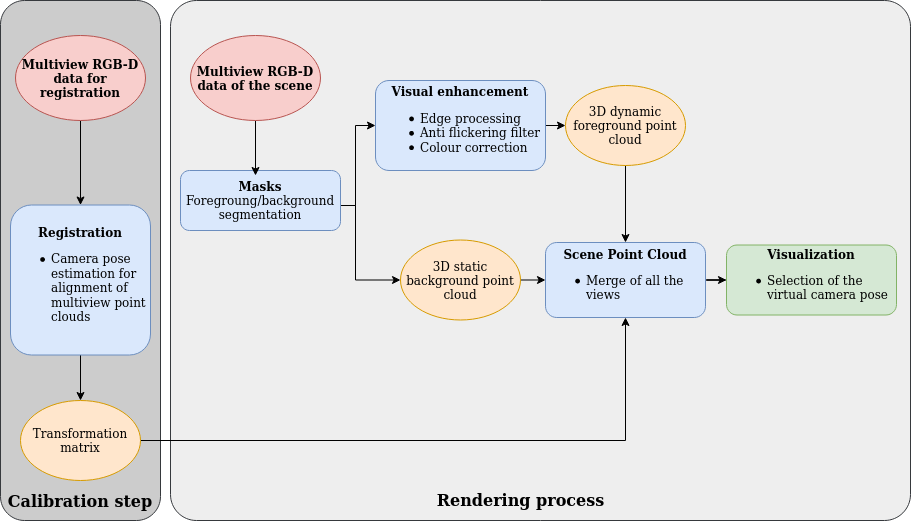
\includegraphics[width=0.95\textwidth]{images/proposed_pipeline_v3.png}
    \caption{Proposed system}
    \label{figure:proposed_pipeline}
\end{figure}